% Dies ist die Main-Datei. Hier werden alle Kapitel zusammengefügt. Hier wird kein Inhalt niedergeschrieben.

% Festlegung des Dokumenttyps und Import von Paketen, die üblicherweise benötigt werden.
\documentclass[11pt]{scrreprt}
\usepackage[left=25mm,right=25mm,top=25mm,bottom=25mm]{geometry}
\usepackage[utf8]{inputenc}
\usepackage[ngerman]{babel}
\usepackage{float}
\usepackage{graphicx}
\usepackage{textcomp, gensymb}
\usepackage{caption}
\usepackage{xcolor}
\usepackage{url}
\usepackage[hidelinks]{hyperref} % Einbinden von Links und Metadaten, farbige Umrandung von Links ist ausgeschalten
\usepackage{varioref}
\usepackage{mathtools}
\usepackage{amssymb}
\usepackage{siunitx}
\usepackage[version=4]{mhchem}
\usepackage{cleveref}
\usepackage{import}
\usepackage{pdfpages}
\usepackage{tikz}
\usepackage{booktabs} % Schönere Tabellen
\usepackage{pgfplots} \pgfplotsset{compat=1.16} % Plotten, Tabellen und vieles mehr

% Verhindert Einrückungen von Text im Dokument
\setlength\parindent{0pt}

% Start des Dokuments
\begin{document}

\pagenumbering{arabic} % Ab hier beginnt die Seitennummerierung.
\setcounter{page}{1}   % mit Seitenzahl 1.

%Ab hier werden die verschiedenen Dateien, aus denen sich das Dokument zusammenfügt, eingebunden.
%--------Deckblatt Versuchsprotokoll----------%
\import{chapters/}{Deckblatt}
%---------------------------------------------%

%--------Inhaltsverzeichnis, Tabellen- und Abbildungsverzeichnis----------%
\setcounter{chapter}{-1} 
\tableofcontents % Erstellt ein Inhaltsverzeichnis
%\vspace{50px}   
%\listoffigures  % Erstellt ein Abbildungsverzeichnis. Dies wird von manchen Tutor*innen gefordert.
%\vspace{50px}   
%\listoftables  % Erstellt ein Tabellenverzeichnis. Dies wird von manchen Tutor*innen gefordert.
\pagebreak
%-------------------------------------------------------------------------%

%--------Aufgabenblatt----------%
%\addcontentsline{toc}{chapter}{Preparation} %kann so dem Inhaltsverzeichnis hinzugefügt werden
%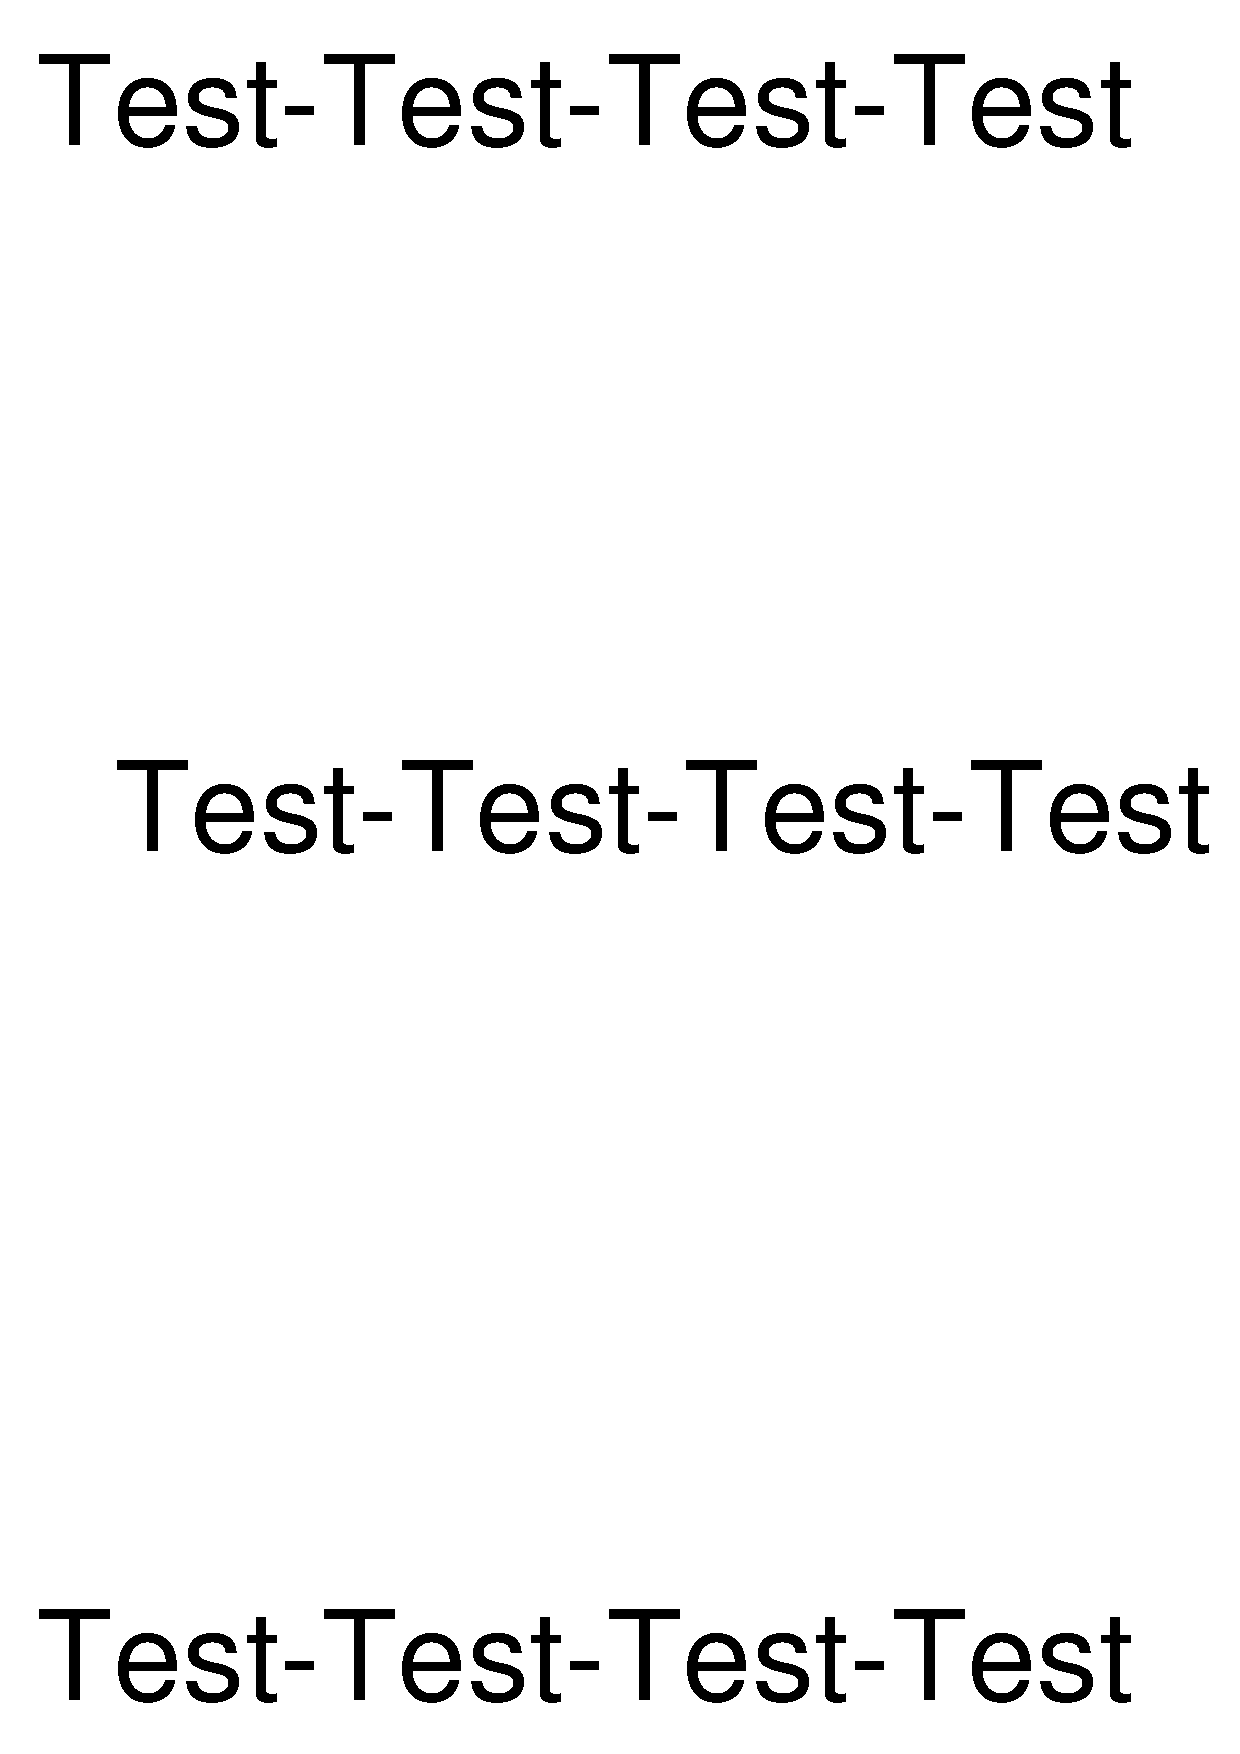
\includepdf[pages=-, pagecommand={}]{include/Aufgabenblatt.pdf} 
% Die Datei Aufgabenblatt.pdf mit dem Inhalt "Test-Test-Test-Test" muss durch das aktuelle Aufgabenblatt des Versuchs ausgetauscht werden.  Der Dateiname muss gleich bleiben oder im \includepdf Befehl geändert werden.
%-------------------------------%



%--------Inhalt der Kapitel----------%

\import{chapters/}{Vorbereitung}

\import{chapters/}{01}

\import{chapters/}{02}

\import{chapters/}{03}

\import{chapters/}{04}

% Werden mehr Aufgabenkapitel benötigt, können diese hier eingebunden werden. \import{chapters/}{Dateiname}
% Zusätzlich muss eine neue *.tex Datei mit dem genannten Dateinamen unter chapters eingefügt werden.
%------------------------------------%

%--------Quellen----------%
\import{chapters/}{Quellen}
%-------------------------%

%--------Anhang (Messprotokoll)----------%
\newpage
\addcontentsline{toc}{chapter}{Messprotokoll}
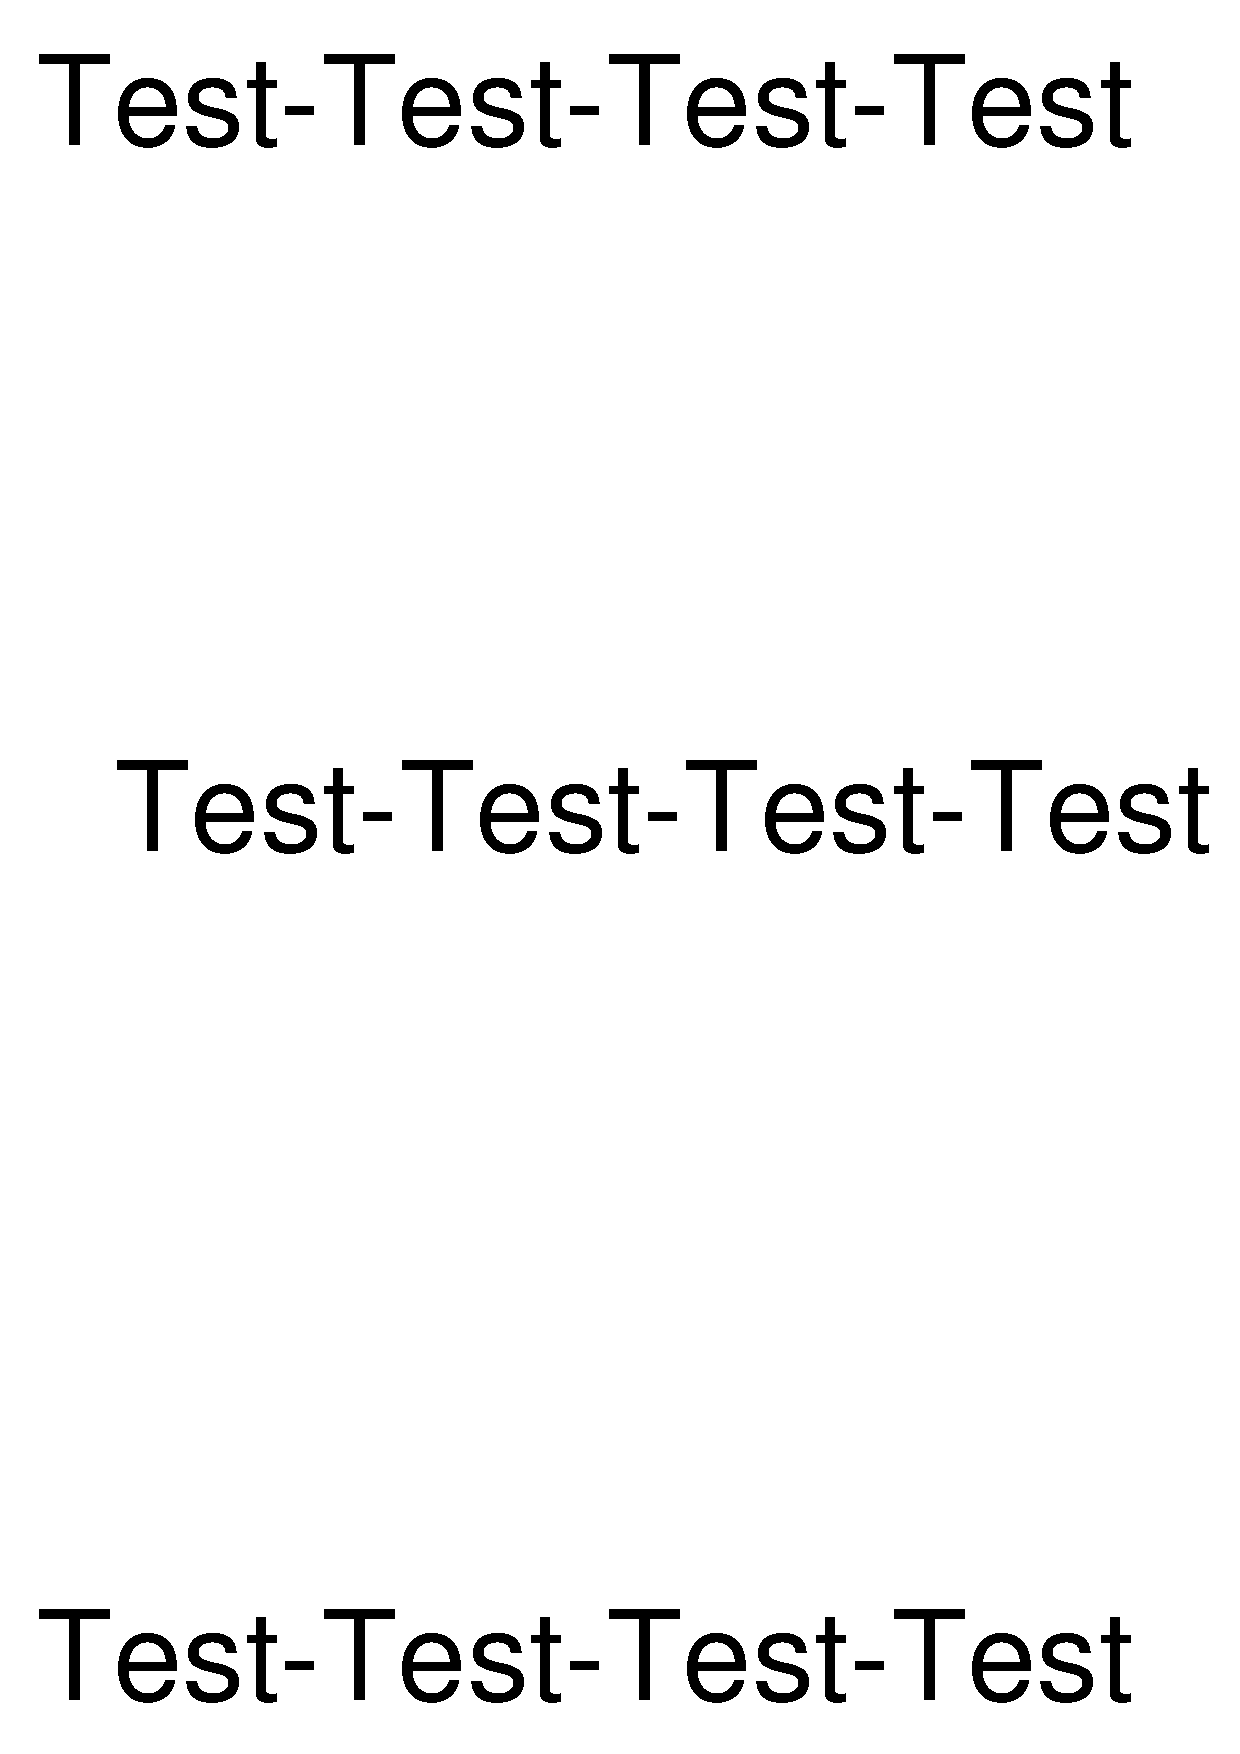
\includepdf[pages=-,pagecommand={}]{include/Messprotokoll.pdf} 
% Die Datei Messprotokoll.pdf mit dem Inhalt "Test-Test-Test-Test" muss durch das, während des Versuchs erstelltem Messprotokoll, ausgetauscht werden.  Der Dateiname muss gleich bleiben oder im \includepdf Befehl geändert werden.
%----------------------------------------%


\end{document}